\documentclass[12pt]{article}
 
\usepackage{afterpage,amssymb,amsmath,amsfonts,eurosym,geometry,
ulem,graphicx,caption,subcaption,color,setspace,sectsty,comment,fnpct,caption,natbib,array,hyperref,float,pdfpages,fancyhdr,pdflscape,amsmath,mathtools,fancyvrb}
\usepackage{xurl}
\usepackage[dvipsnames]{xcolor}
\usepackage[bottom]{footmisc}
\usepackage{booktabs}
\usepackage{pdflscape}
\usepackage{afterpage}
\usepackage{setspace}
\usepackage{longtable}
\usepackage{array}
\usepackage{color}
	\definecolor{maroon}{RGB}{128,0,0}
	\definecolor{navy}{RGB}{0,0,165}
	\definecolor{lb}{RGB}{150,165,190}
    \definecolor{dg}{RGB}{15,92,18}
    \definecolor{purple}{RGB}{145,40,190}
\usepackage{hyperref}
\hypersetup{
     colorlinks = true,
     citecolor = navy,
     linkcolor = navy,
     urlcolor=navy
}

\fancypagestyle{appstyle}{
 \fancyhf{}
 \fancyfoot[C]{\thepage}
 \fancyhead[C]{\textit{Online Appendix}}
}
  
\normalem
\newcommand{\source}[1]{\\ \raggedright {#1}}
\geometry{left=1.0in,right=1.0in,top=1.0in,bottom=1.0in}
 
\newtheorem{theorem}{Theorem}
\newtheorem{acknowledgement}[theorem]{Acknowledgement}
\newtheorem{algorithm}[theorem]{Algorithm}
\newtheorem{axiom}[theorem]{Axiom}
\newtheorem{case}[theorem]{Case}
\newtheorem{claim}[theorem]{Claim}
\newtheorem{conclusion}[theorem]{Conclusion}
\newtheorem{condition}[theorem]{Condition}
\newtheorem{conjecture}[theorem]{Conjecture}
\newtheorem{corollary}[theorem]{Corollary}
\newtheorem{criterion}[theorem]{Criterion}
\newtheorem{definition}[theorem]{Definition}
\newtheorem{example}[theorem]{Example}
\newtheorem{exercise}[theorem]{Exercise}
\newtheorem{lemma}[theorem]{Lemma}
\newtheorem{notation}[theorem]{Notation}
\newtheorem{problem}[theorem]{Problem}
\newtheorem{proposition}[theorem]{Proposition}
\newtheorem{remark}[theorem]{Remark}
\newtheorem{solution}[theorem]{Solution}
\newtheorem{summary}[theorem]{Summary}
\newenvironment{proof}[1][Proof]{\noindent\textbf{#1.} }{\ \rule{0.5em}{0.5em}}

\usepackage[font={large,sc}]{caption}
\usepackage[sc]{mathpazo}
\usepackage[T1]{fontenc}
\VerbatimFootnotes 

\setlength{\tabcolsep}{8pt} % Default value: 6pt
\renewcommand{\arraystretch}{1.5} 
%\newcolumntype{G}{@{\extracolsep{12pt}}c@{\extracolsep{12pt}}}%

\title{QFM Exploration Notes}
\author{}
\date{\today}

\def\cei^#1_#2{\lower\fontdimen17\textfont2\vbox{%
   \baselineskip=\fontdimen17\textfont2 \advance\baselineskip by\fontdimen14\textfont2
   \halign{\hfil$\scriptstyle##$\hfil\cr#1\cr#2\cr}%
}}

\newcommand{\N}{\mathbb{N}}
\newcommand{\Z}{\mathbb{Z}}
\newcommand{\Ztilde}{\mathbf{\Tilde{Z}}}
\newcommand{\E}{\mathbb{E}}

\DeclareMathOperator*{\argmax}{\text{arg} \max}
\DeclareMathOperator*{\argmin}{\text{arg} \min}

\begin{document}

\newgeometry{left=1.0in,right=1.0in,top=1.0in,bottom=1.0in}
\maketitle

\section{Location-Scale Model Notes}

I consider the following DGP:

\begin{equation*}
	y_{it} = \alpha_i\beta_t + \eta_i\gamma_te_{it}
\end{equation*}

\noindent We require that $\eta_t\gamma_t > 0$, so we will draw them from the $\chi^2$ distribution. All together we have:

\[
	\alpha_i \sim \mathcal{N}(0, 1); \quad \beta_t \sim \mathcal{N}(0, 1); \quad \eta_i \sim \chi^2(1); \quad \gamma_t \sim \chi^2(1); \quad e_{it} \sim \mathcal{N}(0,1)
\]

In general, we let $F$ be the cdf of $e_{it}$. Then the conditional quantile function is:

%
\begin{equation*}
	Q_{\tau }(y_{it}|\alpha_i, \beta_t, \eta_i\gamma_t)=\alpha_i\beta_t + \eta_i\gamma_t F^{-1}(\tau)= \alpha_i\beta_t + \eta_i\gamma_t Q(\tau)
\end{equation*}
%

We call the estimates of this conditional quantile function from the QPC algorithm $\hat{\alpha}, \hat{\beta}, \hat{\eta}, \hat{\gamma}$. If the algorithm converges to the true values (as captured by the common component), we would expect that the estimated factors span the same space as the true ones. Because the rotation of the factors is not identified, we need to measure this in a way that is invariant to rotation. To do so, we consider the $R^2$ of the following regressions:

\begin{equation*}
	\beta = a + b_1\hat{\beta} + b_2\hat{\gamma}; \quad \gamma = c + d_1\hat{\gamma} + d_2\hat{\gamma};
\end{equation*}

If the algorithm is converging properly, we would expect high values of $R^2$ in each of these regressions.

Note that under this DGP, beacuse $e_it$ is $\mathcal{N}(0, 1)$ we have that at the median $(\tau = 0.50)$ there will only be one factor.  

For now, I will consider the errors-in-variables rotation, where with $k_{\tau}$ factors, the factor loadings are restricted such that $\Lambda = \left[I_{k_{\tau}} \space \Lambda_2\right]^{\prime}$. This is the most simple computationally, though there are others I could consider from \citet{BaiNg2013}.

For now, I want to see how this DGP behaves and wether we can do any estimation consistently. My target is to replicate table 2 from \citet{Sagner2019}, shown in Figure \ref{fig:sagner_t2}.

\afterpage{%
    \clearpage% Flush earlier floats (otherwise order might not be correct)
    \thispagestyle{empty}% empty page style (?)
    \begin{landscape}% Landscape page
        \begin{figure}[ht]
            \centering
            \caption{}
            \label{fig:sagner_t2}
            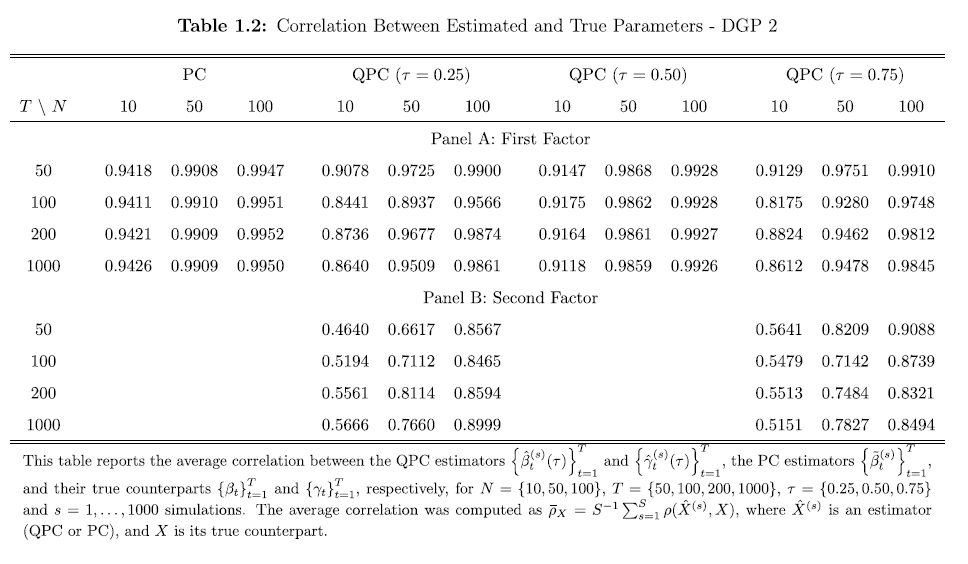
\includegraphics[width=0.9\linewidth]{../out/sagner_t2.png}
        \end{figure}
    \end{landscape}
    \clearpage% Flush page
}

I will not report PC estimates. In addition to the mean $R^2$ values for both the first and second factor, I will include the proportion of simulations where the process took a long time to converge ($> 100$ iterations), where it didn't converge at all (not converged at $1000$ iterations), the proportion of simulations where the $R^2$ for the second factor is $> 0.5$, and the proportion of simulations where the $R^2$ of the first factor is $< 0.9$. For small $N$ and $T$ this last value may be sizable, but for larger $N$ and $T$ a large value of this proportion is concerning as it implies that the first factor is not being estimated consistently.

I want to first check that my estimation procedure is working correctly. To do so, I will consider 2 simple DGPs:

\begin{align}
    y_{it} &= \alpha_i\beta_t + e_{it} \label{eq:dgp1} \\ 
    y_{it} &= \alpha_i\beta_t + \eta_i\gamma_t + e_{it} \label{eq:dgp2}
\end{align}

\noindent These DGPs are simple location models, and so we should expect a good fit for both the one factor case (Equation \ref{eq:dgp1}) and the two factor case (Equation \ref{eq:dgp2}). Results of a small simulation study are reported in. 


\pagebreak \newpage
\singlespacing
%\setlength \bibsep{0pt}
\bibliographystyle{harvard}
%\bibliographystyle{humannat}
\bibliography{literature}

\end{document}


























